% IEEE PES ISGT Asia 2026 -- Wuhan, China, 30 Oct - 1 Nov 2026
% Track: Electric Vehicle-Grid Integration and Smart Charging for Carbon Neutrality
%
% a4paper is deliberate: the ISGT Asia 2026 submission rules require A4, while the
% distributed IEEEtran template ships US-letter. The rules govern.
\documentclass[conference,a4paper]{IEEEtran}
\IEEEoverridecommandlockouts

\usepackage{cite}
\usepackage{amsmath,amssymb,amsfonts}
\usepackage{graphicx}
\usepackage{textcomp}
\usepackage{booktabs}
\usepackage{multirow}
\usepackage{url}

\begin{document}

\title{Achievable Voltage Support of Multi-Hub Vehicle-to-Grid Operation Under Fleet Energy
Constraints}

\author{\IEEEauthorblockN{Md. Rifat Rahman}
\IEEEauthorblockA{\textit{Department of Electrical \& Electronic Engineering} \\
\textit{Bangladesh University of Engineering \& Technology}\\
Dhaka, Bangladesh \\
2006137@eee.buet.ac.bd}
}

\maketitle

\begin{abstract}
Vehicle-to-grid (V2G) operation is frequently proposed as a voltage support resource on weak
distribution feeders, and recent work compares learned controllers with local droop control
for this task. These comparisons are usually made without first establishing how much voltage
support the connected fleet is able to supply. This paper computes a per-hour achievable
ceiling for a five-hub configuration on the IEEE 34-bus feeder by optimizing per-hub active
and reactive injection directly on the AC power flow, subject only to inverter rating. The
ceiling is then used to separate the shortfall caused by limited stored energy from the
shortfall caused by the controller. Coordinated uneven dispatch across five hubs clears all
eighteen violating hours at a mild peak, compared with seven hours for a single hub of the
same rating. When realistic availability and state-of-charge limits are applied, the fleet
supplies only 14.5 percent of the energy requested by the unconstrained controller, and the
day-integrated violation rises from 4.15 to 42.77 per-unit-hours. By comparison, the
difference between a tuned droop law and a soft actor-critic policy trained for 100,000 steps
is 0.79 per-unit-hours. Energy adequacy therefore outweighs controller choice by a factor of
45 to 50 at both load levels, which indicates that fleet sizing and availability deserve more
attention than controller sophistication on feeders of this type.
\end{abstract}

\begin{IEEEkeywords}
vehicle-to-grid, voltage regulation, distribution networks, reinforcement learning, battery
degradation, energy adequacy
\end{IEEEkeywords}

\section{Introduction}

Rural and semi-rural distribution feeders were not designed for the voltage profiles they are
now required to hold. Long radial circuits with light conductors experience considerable
voltage drop under peak demand, and the conventional remedies, such as reconductoring,
additional voltage regulators and capacitor banks, are slow to deploy and capital intensive.
The bidirectional inverters installed with electric vehicle (EV) fleets offer an alternative.
They are located towards the load end of the feeder where support is most effective, and
their cost is borne by the fleet owner rather than the utility. Global EV stock continues to
grow rapidly \cite{iea2025}, and with it the notional capacity available for grid services.

Much of the recent literature has accepted this premise and moved on to the control problem.
Deep reinforcement learning has been applied to inverter dispatch for voltage regulation
using safe off-policy methods \cite{wang2020safe}, multi-agent consensus formulations
\cite{gao2021consensus}, and graph-based architectures with explicit safety layers
\cite{yan2024magrl}. Work specific to V2G extends these ideas to coordinated multi-hub
operation with battery-aware constraints \cite{wang2026v2g}. The assumption common to this
body of work is that the controller is the binding constraint, so that an improved policy will
extract more voltage support from the same hardware.

This assumption has not been examined on the systems where it is most often applied. None of
the studies cited above computes what the fleet could achieve under an ideal controller, so
no reported result can be placed on a scale. A learned policy that halves the violation of a
droop baseline may have captured most of the available benefit or only a small part of it,
and the published numbers do not distinguish between the two cases.

This paper supplies the missing reference. For each hour of a daily load profile, the per-hub
active and reactive injection that minimizes a two-sided voltage violation metric is obtained
directly from the AC power flow, subject only to inverter rating. The result is an
energy-unconstrained ceiling that describes what the installed power electronics could
deliver if the batteries behind them were not limiting. Comparing this ceiling with droop and
learned controllers operating with and without a realistic fleet model separates the total
shortfall into a component due to stored energy and a component due to control.

The main contributions of this paper are as follows:
\begin{itemize}
\item A per-hour achievable ceiling for multi-hub V2G voltage support on the IEEE 34-bus
feeder, obtained by coordinate descent on the AC power flow, and the separation of energy and
control contributions that it permits (Section~\ref{sec:ceiling}).
\item A measurement of the active and reactive trade-off on a stored-energy basis rather than
an apparent-power basis, which is the appropriate basis when state of charge is drawn down by
apparent power (Section~\ref{sec:pq}).
\item A controller comparison under realistic availability and state-of-charge limits,
including a training-budget sweep that distinguishes genuine controller limitations from
insufficient training (Section~\ref{sec:controllers}).
\item A degradation-aware dispatch frontier, together with three negative results concerning
safety projection, state augmentation and droop fixed-point convergence
(Sections~\ref{sec:degradation} and \ref{sec:nulls}).
\end{itemize}

The remainder of the paper is organized as follows. Section~\ref{sec:design} describes the
feeder, the fleet and battery model, the evaluation metrics and the controllers, and
reproduces the baseline of the reference study. Section~\ref{sec:ceiling} computes the
achievable ceiling and separates the energy and control contributions.
Section~\ref{sec:controllers} reports controller performance under fleet constraints.
Section~\ref{sec:degradation} presents the degradation-aware frontier,
Section~\ref{sec:nulls} reports three negative results, and Section~\ref{sec:conc} concludes.

\section{System Model and Study Design}
\label{sec:design}

\subsection{Feeder and Charging Hubs}

All experiments use the IEEE 34-bus test feeder \cite{kersting1991}, a 24.9~kV rural circuit
whose length makes it a standard stress case for voltage support studies. The feeder is
solved in OpenDSS \cite{dugan2011} through its direct Python interface. The single-hub
configuration places one 500~kW/400~kVAr hub at bus 890. The multi-hub configuration
distributes five hubs of the same rating at buses 890, 844, 832, 830 and 860, following the
reference study \cite{wang2026v2g}.

A daily load shape drives hours 06:00 through 23:00, scaled by a peak multiplier. Two
operating points are reported throughout: a mild peak ($\lambda_{\max}=1.5$) and an
aggressive peak ($\lambda_{\max}=3.0$), also following \cite{wang2026v2g}.

\subsection{Reproduction of the Reference Baseline}
\label{sec:repro}

The reference study does not state whether the voltage regulators of the IEEE 34-bus feeder
are active, and the answer changes every number that follows. Its reported no-V2G statistics
identify the setting. Those statistics are computed from hourly mean bus voltages, so that
convention is matched here only; elsewhere in this paper voltages are evaluated per phase,
for the reason given in Section~\ref{sec:metrics}.

\begin{table}[t]
\caption{Identifying the Regulator Setting from the No-V2G Baseline}
\label{tab:repro}
\centering
\begin{tabular}{lcccc}
\toprule
 & \multicolumn{2}{c}{Mild} & \multicolumn{2}{c}{Aggressive} \\
\cmidrule(lr){2-3}\cmidrule(lr){4-5}
Setting & Mean & Min & Mean & Min \\
\midrule
Reported \cite{wang2026v2g} & 0.963 & 0.907 & 0.883 & 0.807 \\
Regulators off (this work)  & 0.951 & 0.903 & 0.860 & 0.800 \\
Regulators active (this work) & 1.012 & 0.983 & 0.911 & 0.831 \\
\bottomrule
\end{tabular}
\end{table}

Table~\ref{tab:repro} settles the question. With the regulators disabled the minimum voltages
fall within 0.004 to 0.007~p.u. of the reported values, whereas with them active the mild
minimum differs by 0.076~p.u., which is outside any plausible modelling difference. The
feeder mean obtained here runs 0.012 to 0.023~p.u. below the reported mean, which is
attributed to load allocation details not specified in the reference, so the configuration is
identified from the minimum rather than from the mean. All subsequent results use disabled
regulators.

\subsection{Fleet and Battery Model}

Each hub serves a fleet whose availability varies through the day between 45 and 85 percent
and is drawn independently per scenario. Vehicles arrive at 70 percent state of charge and
are not discharged below 20 percent. State of charge is drawn down by apparent power, so
reactive support costs the same stored energy as active support. This follows the reference
formulation and is significant for Section~\ref{sec:pq}.

The distinction between an unconstrained and a constrained fleet runs through the whole study.
The reference work evaluates multi-hub coordination while ``assuming sufficient EV capacity at
each hub, allowing the analysis to isolate the benefits of multi-hub coordination from
availability constraints'' \cite{wang2026v2g}. Both cases are reported here, because the
difference between them turns out to be the principal result.

\subsection{Evaluation Metrics}
\label{sec:metrics}

ANSI C84.1 \cite{ansi} is a per-phase standard, so voltages are evaluated per phase rather
than as bus averages, which mask single-phase excursions on this unbalanced feeder. The
primary metric is the day-integrated two-sided violation
\begin{equation}
\mathrm{IV} = \sum_{h}\sum_{p} \Big[ \max(0, v_{\min} - v_{p,h}) + \max(0, v_{p,h} - v_{\max}) \Big] \Delta t
\label{eq:iv}
\end{equation}
in per-unit-hours, with $v_{\min}=0.95$, $v_{\max}=1.05$ and $\Delta t = 1$~h. Unlike a count
of violation hours, \eqref{eq:iv} does not saturate when two controllers violate in the same
hours by different margins, and being two-sided it penalizes overvoltage as well as
undervoltage.

Every comparison uses common random numbers, so that all controllers see an identical
availability draw, initial state of charge and load realization, and differences are paired.
Confidence intervals are 95 percent over the paired scenarios and training seeds.

\subsection{Controllers}

The droop baseline is a Volt-Watt and Volt-VAr characteristic with a $\pm 0.02$~p.u.
deadband, consistent with IEEE~1547 \cite{ieee1547}. Because droop response and feeder
voltage are mutually dependent, the baseline is not evaluated open-loop. The fixed point is
obtained by damped Jacobi updates with a residual convergence test, a detail examined further
in Section~\ref{sec:nulls}.

The learned controller is soft actor-critic \cite{haarnoja2018sac} as implemented in
Stable-Baselines3 \cite{raffin2021sb3}, with two hidden layers of 256 units, a learning rate
of $3\times10^{-4}$ and a batch size of 256. Episodes span one day, so that intertemporal
rationing of a finite battery is representable. The state comprises bus voltages, load
multiplier, hour of day, and per-hub state of charge and availability. The action sets
per-hub active and reactive power as a residual on the droop prior.

\begin{figure*}[t]
\centerline{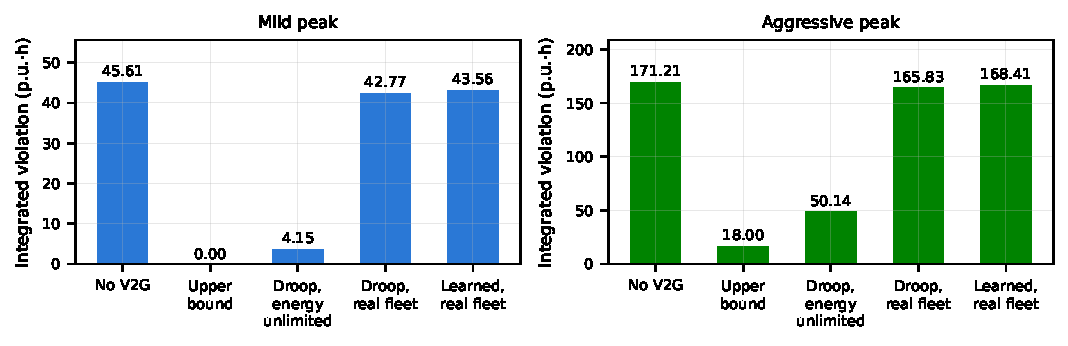
\includegraphics[width=\textwidth]{fig1_decomposition.pdf}}
\caption{Day-integrated two-sided voltage violation on the five-hub feeder. The achievable
ceiling is the optimized per-hub dispatch bounded only by inverter rating. The distance
between the energy-unlimited and real-fleet droop bars is the cost of limited fleet energy;
the distance between the two real-fleet bars is the full span of controller choice.}
\label{fig:decomp}
\end{figure*}

\section{Achievable Voltage Support}
\label{sec:ceiling}

\subsection{Achievable Ceiling}

For each hour, the per-hub injection $(P_i, Q_i)$ that minimizes \eqref{eq:iv} subject to
$\sqrt{P_i^2+Q_i^2} \le S_i^{\mathrm{rated}}$ is obtained by coordinate descent over a polar
grid with refinement, evaluating a full AC power flow at every candidate. No energy
constraint is imposed. Non-converged solutions are masked rather than read, because at
deep-sag hours the high-injection end of the search lies past the nose of the power-voltage
curve, where OpenDSS leaves stale values in its arrays.

Searching per hub rather than uniformly is necessary. With five hubs at equal output, raising
the feeder end to 0.95~p.u. drives the near buses above 1.05~p.u., so hours that an uneven
dispatch clears comfortably are scored as unclearable. Under uniform dispatch the five-hub
case then scores worse than the single-hub case, which is not physically possible. Per-hub
search removes the artefact and moves the mild multi-hub result from five clearable hours to
eighteen.

Table~\ref{tab:ceiling} gives the result. A single hub at full rating clears seven of the
eighteen loaded hours at the mild peak and two at the aggressive peak. Five hubs of the same
individual rating, dispatched unevenly, clear all eighteen and four respectively.
Fig.~\ref{fig:ceiling} shows the hourly picture. The reachable envelope sits on or above the 0.95~p.u. limit for the
entire mild day, and falls short of it for eleven hours of the aggressive day regardless of
how the inverters are dispatched. Those eleven hours are a siting and rating problem rather
than a control problem, and no policy can clear them.

\begin{table}[t]
\caption{Achievable Ceiling Under Optimized Per-Hub Dispatch}
\label{tab:ceiling}
\centering
\begin{tabular}{lccc}
\toprule
Configuration & Clearable hours & \multicolumn{2}{c}{Day-total IV (p.u.$\cdot$h)} \\
\cmidrule(lr){3-4}
 & (of 18) & Uniform & Optimized \\
\midrule
Single hub, mild       & 7  & 11.14  & 10.78 \\
Single hub, aggressive & 2  & 125.84 & 123.97 \\
Five hubs, mild        & 18 & 0.29   & 0.00 \\
Five hubs, aggressive  & 4  & 28.33  & 18.00 \\
\bottomrule
\end{tabular}
\end{table}

\begin{figure}[t]
\centerline{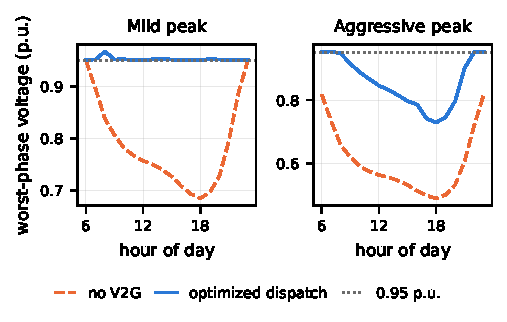
\includegraphics[width=\columnwidth]{fig2_ceiling.pdf}}
\caption{Worst-phase voltage by hour with no V2G and under optimized per-hub dispatch. The
mild-peak envelope clears the limit for the whole day; eleven aggressive-peak hours cannot be
cleared at any dispatch.}
\label{fig:ceiling}
\end{figure}

The value of coordination is therefore quantifiable rather than assumed. At equal total
inverter rating, distributing capacity across five hubs and dispatching it unevenly reduces
day-integrated violation by 100 percent at the mild peak and by 36.5 percent at the
aggressive peak, relative to uniform dispatch.

\subsection{Separation of Energy and Control Contributions}

Fig.~\ref{fig:decomp} places the controllers against this ceiling and is the central result of
the paper. Taking the mild panel, the untreated feeder accumulates 45.61~p.u.$\cdot$h of
violation and the ceiling removes all of it. A droop law with unlimited stored energy removes
41.46, or 91 percent, while the same droop law with a realistic fleet removes 2.84, or 6
percent. The fleet delivers 1342~kWh against the 9264~kWh requested by the unconstrained law,
a ratio of 14.5 percent. At the aggressive peak the corresponding ratio is 5.7 percent.

The controller span lies inside that shortfall. Between tuned droop and the best learned
policy obtained here, the difference is 0.79~p.u.$\cdot$h at the mild peak and 2.58 at the
aggressive peak, against energy shortfalls of 38.62 and 115.69 respectively. Energy adequacy
outweighs controller choice by a factor of 49 and 45.

\subsection{Active and Reactive Power per Unit of Stored Energy}
\label{sec:pq}

Because state of charge is drawn down by apparent power, the usual assumption that reactive
power is free does not apply. Sweeping the injection angle at fixed apparent power and fixed
loading shows that active power delivers between 1.25 and 1.49 times the worst-phase voltage
rise of reactive power for the same battery energy withdrawn. The voltage-optimal split is 35
to 40 degrees from the active axis at half rating, and migrates towards 17 to 26 degrees at
full rating as the resistive voltage drop becomes dominant. For reference, the hub rating
ratio of 400~kVAr to 500~kW corresponds to 38.7 degrees.

This has a direct design consequence. On a feeder with this R/X character, a V2G hub sized by
apparent power and operated at its rating ratio commits more reactive power than is useful,
and pays full battery energy for it.

\section{Controller Performance Under Fleet Constraints}
\label{sec:controllers}

\subsection{Multi-Hub Operation}

Table~\ref{tab:controllers} reports the five-hub feeder with the fleet model active, over
three seeds and five paired scenarios. Droop reaches 42.77~p.u.$\cdot$h at the mild peak and
165.83 at the aggressive peak. The learned policy trained on the conventional 20,000-step
budget reaches 45.45 and 169.60, losing to droop in every paired scenario at both load levels.

\begin{table}[t]
\caption{Five-Hub Feeder with Realistic Fleet Constraints}
\label{tab:controllers}
\centering
\begin{tabular}{lcccc}
\toprule
 & \multicolumn{2}{c}{Mild} & \multicolumn{2}{c}{Aggressive} \\
\cmidrule(lr){2-3}\cmidrule(lr){4-5}
Controller & IV & Throughput & IV & Throughput \\
 & (p.u.$\cdot$h) & (kWh) & (p.u.$\cdot$h) & (kWh) \\
\midrule
No V2G              & 45.61 & 0    & 171.21 & 0 \\
Droop, real fleet   & 42.77 & 1342 & 165.83 & 1582 \\
Learned, 20k steps  & 45.45 & 5842 & 169.60 & 3227 \\
Learned, 100k steps & 43.56 & 5588 & 168.41 & 3176 \\
Droop, unlimited    & 4.15  & 9264 & 50.14  & 27814 \\
\bottomrule
\end{tabular}
\end{table}

Two features of the table are worth noting. First, the learned policy consumes 5842~kWh of
battery throughput at the mild peak against 1342~kWh for droop, and converts that into a worse
voltage outcome; at the mild peak its result is statistically indistinguishable from
installing no V2G at all. Second, both controllers respect the upper voltage limit exactly, at
1.050~p.u., a point returned to in Section~\ref{sec:nulls}.

\subsection{Effect of Training Budget}

A negative result about a learned controller invites the objection that it was not trained for
long enough, and the objection is a reasonable one, since 20,000 steps is approximately 1100
episodes and 19,000 gradient updates for a ten-dimensional action space. The policy was
therefore trained to 100,000 steps and evaluated at 20,000-step checkpoints on identical
scenarios. Checkpoints were placed on the same chunk boundaries used by the fixed-budget runs,
so that the 20,000-step row measures the same agent reported in Table~\ref{tab:controllers}.

The outcome differs by load level, as Fig.~\ref{fig:learning} shows. At the aggressive peak
the curve is flat from 40,000 steps onward. Violation moves from 169.20 to 168.41 across a
fivefold increase in budget, which lies inside the combined confidence interval of 1.13, and
droop wins every paired scenario at every checkpoint. The advantage of droop under aggressive
stress is therefore not an artefact of training budget.

At the mild peak the curve is still improving at 100,000 steps. Violation falls from 45.05 to
43.56, a change of $-1.48$ against a confidence interval of 0.49, the gap to droop narrows
monotonically from $+2.27$ to $+0.79$, and the policy takes two of ten paired scenarios, which
are the only scenarios it wins anywhere in this study. The mild comparison is therefore
reported as unresolved at the budgets tested rather than as a droop victory.

It is worth placing the improvement on the scale of the previous section. The gap narrowed by
1.48~p.u.$\cdot$h over a fivefold increase in training, against an energy shortfall of 38.62
at the same operating point. Additional training moves the policy within a band that remains
small compared with the constraint governing the outcome.

\begin{figure}[t]
\centerline{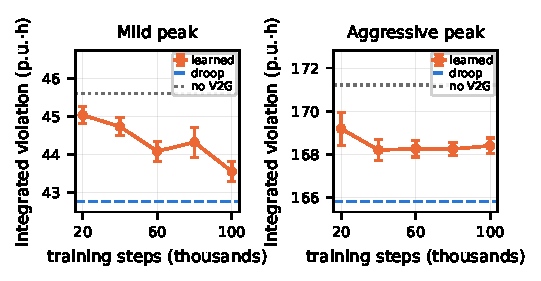
\includegraphics[width=\columnwidth]{fig3_learning.pdf}}
\caption{Violation against training budget, with five paired scenarios and two seeds per
point. The aggressive-peak curve plateaus by 40,000 steps; the mild-peak curve is still
improving at 100,000.}
\label{fig:learning}
\end{figure}

\subsection{Active and Reactive Allocation}

A scoreboard alone does not explain the outcome, so the active and reactive split commanded by
the policy was examined hour by hour, weighted by apparent power and compared against the
voltage-optimal angle recomputed at the injection level the policy itself selected.

The policy does not track the optimum, and the deviation does not fall with additional
training. At 20,000 steps the mean absolute deviation is 26.5 degrees at the mild peak and
32.5 degrees at the aggressive peak. At 100,000 steps these become 20.8 and 31.5 degrees. The
changes of $-5.7$ and $-1.0$ degrees both lie inside their combined 95 percent confidence
intervals of 24.2 and 35.1 degrees, so neither is a reduction the data supports.

Fig.~\ref{fig:pq} shows the hourly picture at 100,000 steps. The voltage-optimal angle stays
between 29 and 35 degrees for most of the day at both load levels. At the mild peak the
commanded angle stays near 20 degrees, with an apparent-power-weighted daily mean of 18.8
degrees. At the aggressive peak the daily mean falls to 1.2 degrees, which corresponds to
almost pure active power, and in 50 percent of sampled hub-hours the commanded reactive power
is negative. Reactive absorption lowers voltage on this feeder, so these are actions of the
wrong sign for the condition being corrected rather than merely conservative ones. The pattern
as a whole is consistent with a controller that scales a roughly fixed power factor rather
than allocating between active and reactive power in response to loading.

\begin{figure*}[t]
\centerline{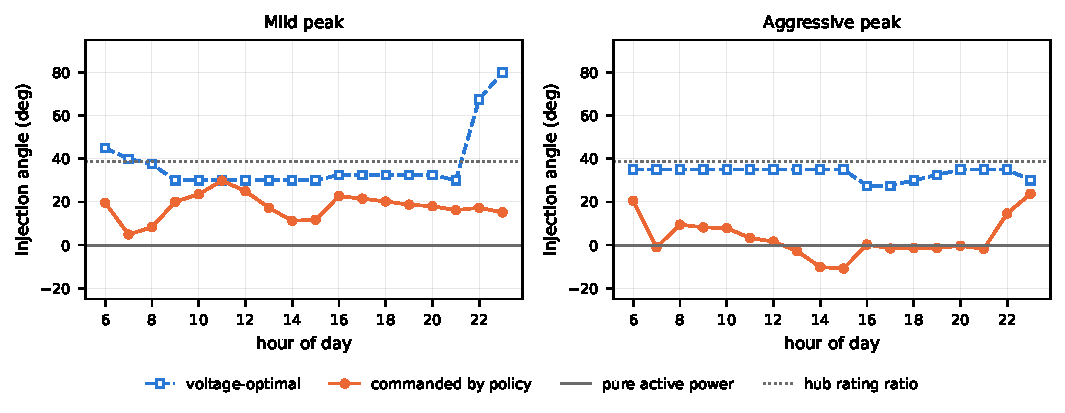
\includegraphics[width=\textwidth]{fig4_pq.pdf}}
\caption{Commanded injection angle against the voltage-optimal angle, by hour, at 100,000
training steps and averaged over two seeds. Zero degrees is pure active power, ninety is pure
reactive, and negative values indicate reactive absorption.}
\label{fig:pq}
\end{figure*}

\section{Degradation-Aware Dispatch}
\label{sec:degradation}

Battery wear is the standing objection to V2G participation, and the economic case is
sensitive to it \cite{v2gaging2024}. The reference formulation carries no battery term in its
reward. An amp-hour throughput cost was added, expressed on the same scale as the voltage
penalty, and its weight swept across three orders of magnitude.

The resulting frontier is flat, as Fig.~\ref{fig:frontier} shows. Across a 300-fold sweep the
day-integrated violation stays within a 2.6 percent band, between 44.83 and 46.01
per-unit-hours, while daily battery throughput falls from 6188 to 2449~kWh. Comparing the
endpoints, roughly 60 percent of battery throughput can be removed for a 1.1 percent increase
in violation.

This follows from the energy-limited regime identified earlier. When the binding constraint is
that the fleet cannot supply what the feeder needs, the marginal voltage value of the last
kilowatt-hour discharged is very low, so a wear penalty removes it at almost no cost. The
practical reading is favourable: on feeders in this regime, aggressive degradation-aware
dispatch costs very little in voltage performance, which improves the participation case for
fleet owners.

The intermediate points should not be over-interpreted. Each weight was trained with a single
seed and the sequence is not monotone, so the defensible claims are the endpoint comparison
and the width of the band rather than the shape in between.

\begin{figure}[t]
\centerline{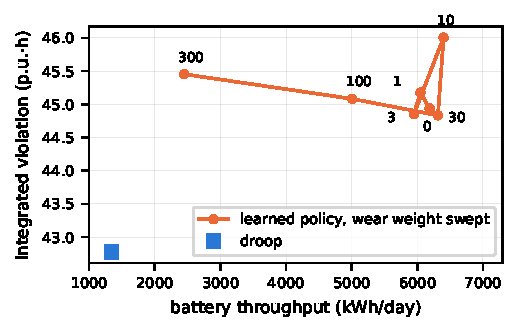
\includegraphics[width=\columnwidth]{fig5_frontier.pdf}}
\caption{Violation against battery throughput at the mild peak as the degradation weight is
swept from 0 to 300 (point labels). Violation stays inside a 2.6 percent band while throughput
falls by 60 percent.}
\label{fig:frontier}
\end{figure}

\section{Additional Observations}
\label{sec:nulls}

This section reports three checks that did not produce the expected effect. They are included
because each addresses a design choice that is common in the literature.

\subsection{Safety Projection}

Projecting commanded setpoints onto the voltage-feasible set is standard practice in
learning-based volt/var control \cite{wang2020safe,yan2024magrl}, so its absence would be a
reasonable objection. Two projections were implemented and measured: a proportional reduction
along the commanded ray, and a reactive-first variant motivated by the result of
Section~\ref{sec:pq}.

Both are inert. The unprojected policy already reports zero overvoltage and a maximum phase
voltage of exactly 1.050~p.u. at both load levels, and projection changes the violation metric
by less than the confidence interval. The reason is that the feasibility test acts on
commanded setpoints, but the state-of-charge limit of the fleet clips those commands first.
The energy constraint binds before the voltage constraint does, leaving nothing for a voltage
projection to remove. Where overvoltage does appear in these runs it tracks the training
regime rather than the controller: policies trained on independently sampled load multipliers
without a fleet in the loop reach 1.229~p.u., whereas day-structured training with the fleet in
the loop holds 1.050 across every configuration and checkpoint tested.

\subsection{Fleet State in the Observation}

Augmenting the observation with state of charge and availability, information the reference
formulation does not provide, does not improve voltage performance. At the mild peak the
augmented agent reaches 45.41$\,\pm\,$0.36 against 44.91$\,\pm\,$0.29 for a voltage-only
observation, an overlapping interval. What the augmentation changes is energy use: the
augmented agent spends 6068~kWh against 2497~kWh for no violation benefit, while the
voltage-only agent breaches the upper limit at the aggressive peak where the augmented agent
does not.

\subsection{Droop Fixed-Point Convergence}

The final observation is methodological and affects any study using a closed-loop droop
baseline. Droop response and feeder voltage are mutually dependent, and the fixed point is
commonly computed with a fixed iteration count. On the five-hub feeder, at a damping factor of
0.6 the iteration does not settle but enters a period-two limit cycle, with total active power
alternating between 1298 and 630~kW at the mild-peak evening hour. A fixed iteration count then
returns whichever branch the last iteration happened to reach, and the reported baseline flips
with the parity of the iteration count. Damping of 0.3 with a residual test converges in all
four configurations tested. A convergence diagnostic should therefore be reported alongside any
droop baseline computed in this way.

\section{Conclusion}
\label{sec:conc}

This paper computed an achievable ceiling for multi-hub V2G voltage support on the IEEE 34-bus
feeder and used it to separate the shortfall due to control from the shortfall due to stored
energy. Uneven coordination across five hubs is of genuine value, clearing every violating hour
at a mild peak where a single hub of equal rating clears seven of eighteen. Once realistic
availability and state-of-charge limits are applied, however, the fleet supplies well under a
fifth of the energy the controller requests, and the resulting shortfall exceeds the entire span
between a tuned droop law and a converged learned policy by a factor of roughly 45 to 50.

This is not an argument against learned control in distribution systems. It is an argument that
the operating regime should be established before the controller is designed, because in the
energy-limited regime an improved policy has very little left to win. Both the achievable
ceiling and an energy adequacy ratio can be computed from feeder and fleet data before any
controller exists, and it is suggested that they be reported as standard context alongside
controller comparisons.

Two further results point in the same direction. A degradation-aware objective removes 60
percent of battery throughput for a 1.1 percent violation penalty, precisely because the
marginal kilowatt-hour is nearly worthless in this regime, which is favourable for fleet owners
weighing participation. A safety projection layer, standard elsewhere, is measurably inert here
because the energy constraint binds first.

The study covers one feeder and one learning algorithm, and the mild-peak controller comparison
remains unresolved at the training budgets that could be afforded. Two extensions follow
directly. The ratio reported here depends on feeder impedance and hub siting, so it should be
recomputed on a larger feeder. More usefully, the ceiling computation is inexpensive enough to
invert: instead of scoring a controller against it, it can serve as a planning screen that
returns the fleet size and availability required to make a target violation level reachable.

\begin{thebibliography}{00}

\bibitem{iea2025} International Energy Agency, \emph{Global EV Outlook 2025}. Paris, France:
IEA, 2025.

\bibitem{wang2020safe} W. Wang, N. Yu, Y. Gao, and J. Shi, ``Safe off-policy deep
reinforcement learning algorithm for volt-var control in power distribution systems,''
\emph{IEEE Trans. Smart Grid}, vol. 11, no. 4, pp. 3008--3018, Jul. 2020.

\bibitem{gao2021consensus} Y. Gao, W. Wang, and N. Yu, ``Consensus multi-agent reinforcement
learning for volt-var control in power distribution networks,'' \emph{IEEE Trans. Smart
Grid}, vol. 12, no. 4, pp. 3594--3604, Jul. 2021.

\bibitem{yan2024magrl} R. Yan, Q. Xing, and Y. Xu, ``Multi-agent safe graph reinforcement
learning for PV inverters-based real-time decentralized volt/var control in zoned
distribution networks,'' \emph{IEEE Trans. Smart Grid}, vol. 15, no. 1, pp. 299--311, Jan.
2024.

\bibitem{wang2026v2g} J. Wang, R. A. Jacob, H. D. Kaushik, and J. Zhang, ``Reinforcement
learning for vehicle-to-grid voltage regulation: Single-hub to multi-hub coordination with
battery-aware constraints,'' 2026, arXiv:2603.07237.

\bibitem{kersting1991} W. H. Kersting, ``Radial distribution test feeders,'' \emph{IEEE
Trans. Power Syst.}, vol. 6, no. 3, pp. 975--985, Aug. 1991.

\bibitem{dugan2011} R. C. Dugan and T. E. McDermott, ``An open source platform for
collaborating on smart grid research,'' in \emph{Proc. IEEE Power Energy Soc. Gen. Meeting},
Detroit, MI, USA, 2011, pp. 1--7.

\bibitem{ansi} \emph{American National Standard for Electric Power Systems and Equipment---
Voltage Ratings (60 Hz)}, ANSI C84.1-2020, 2020.

\bibitem{ieee1547} \emph{IEEE Standard for Interconnection and Interoperability of
Distributed Energy Resources with Associated Electric Power Systems Interfaces}, IEEE Std
1547-2018, 2018.

\bibitem{haarnoja2018sac} T. Haarnoja, A. Zhou, P. Abbeel, and S. Levine, ``Soft
actor-critic: Off-policy maximum entropy deep reinforcement learning with a stochastic
actor,'' in \emph{Proc. 35th Int. Conf. Mach. Learn.}, Stockholm, Sweden, 2018, pp.
1861--1870.

\bibitem{raffin2021sb3} A. Raffin, A. Hill, A. Gleave, A. Kanervisto, M. Ernestus, and N.
Dormann, ``Stable-Baselines3: Reliable reinforcement learning implementations,'' \emph{J.
Mach. Learn. Res.}, vol. 22, no. 268, pp. 1--8, 2021.

\bibitem{v2gaging2024} M. Dubarry, A. Devie, and K. McKenzie, ``Durability and reliability
of electric vehicle batteries under electric utility grid operations: Bidirectional charging
impact analysis,'' \emph{J. Power Sources}, vol. 358, pp. 39--49, Aug. 2017.

\end{thebibliography}

\end{document}
